\section{\rqthree}
\label{results:rq3}

Here we investigate the impact of the composition of program variants into multivariant binaries.
To answer this research question, we create multivariant binaries from the program variants generated for \corpussodium and \corpusqrcode corpora. Then, we deploy the multivariant binaries into the Edge and collect their execution times. 

\subsection*{Timing side-channels.}

We compare the execution time distributions for each program for the original and the multivariant binary. All distributions are measured on 100k executions of the program along all Edge platform nodes.
% statistics
We have observed that the distributions for multivariant binaries have a higher standard deviation of execution time.
A statistical comparison between the execution time distributions confirms the significance of this difference (P-value = 0.05 with a  Mann-Withney U test). This hints at the fact that the execution time for multivariant binaries is more unpredictable than the time to execute the original binary. 


% Curve flatenning
In \autoref{rq3:diversity:times}, each subplot represents the quantile-quantile plot \cite{gnanadesikan1968probability} of the two distributions, original and multivariant binary.
This kind of plots is used to compare the shapes of distributions, providing a graphical comparison of location, scale, and skewness for two distributions.
The dashed line cutting the subplot represents the case in which the two distributions are equal, \ie for two equal distribution we would have all blue dots over the dashed line. These plots reveal that the execution times are different and are spread over a more extensive range of values than the original binary.
The standard deviation of the execution time values evidences the latter, the original binaries have lower values while the multivariant binaries have higher values up to $100$ times the original. Besides, this can be graphically appreciated in the plots when the blue dots cross the reference line from the bottom of the dashed line to the top.
This is evidence that execution time is less predictable for multivariant binaries than original ones.
This phenomenon is present because the choice of function variants is randomized at each function invocation, and the variants have different execution times due to the code transformations, i.e., some variants execute more instructions than others. 
 

\begin{figure*}[h]
    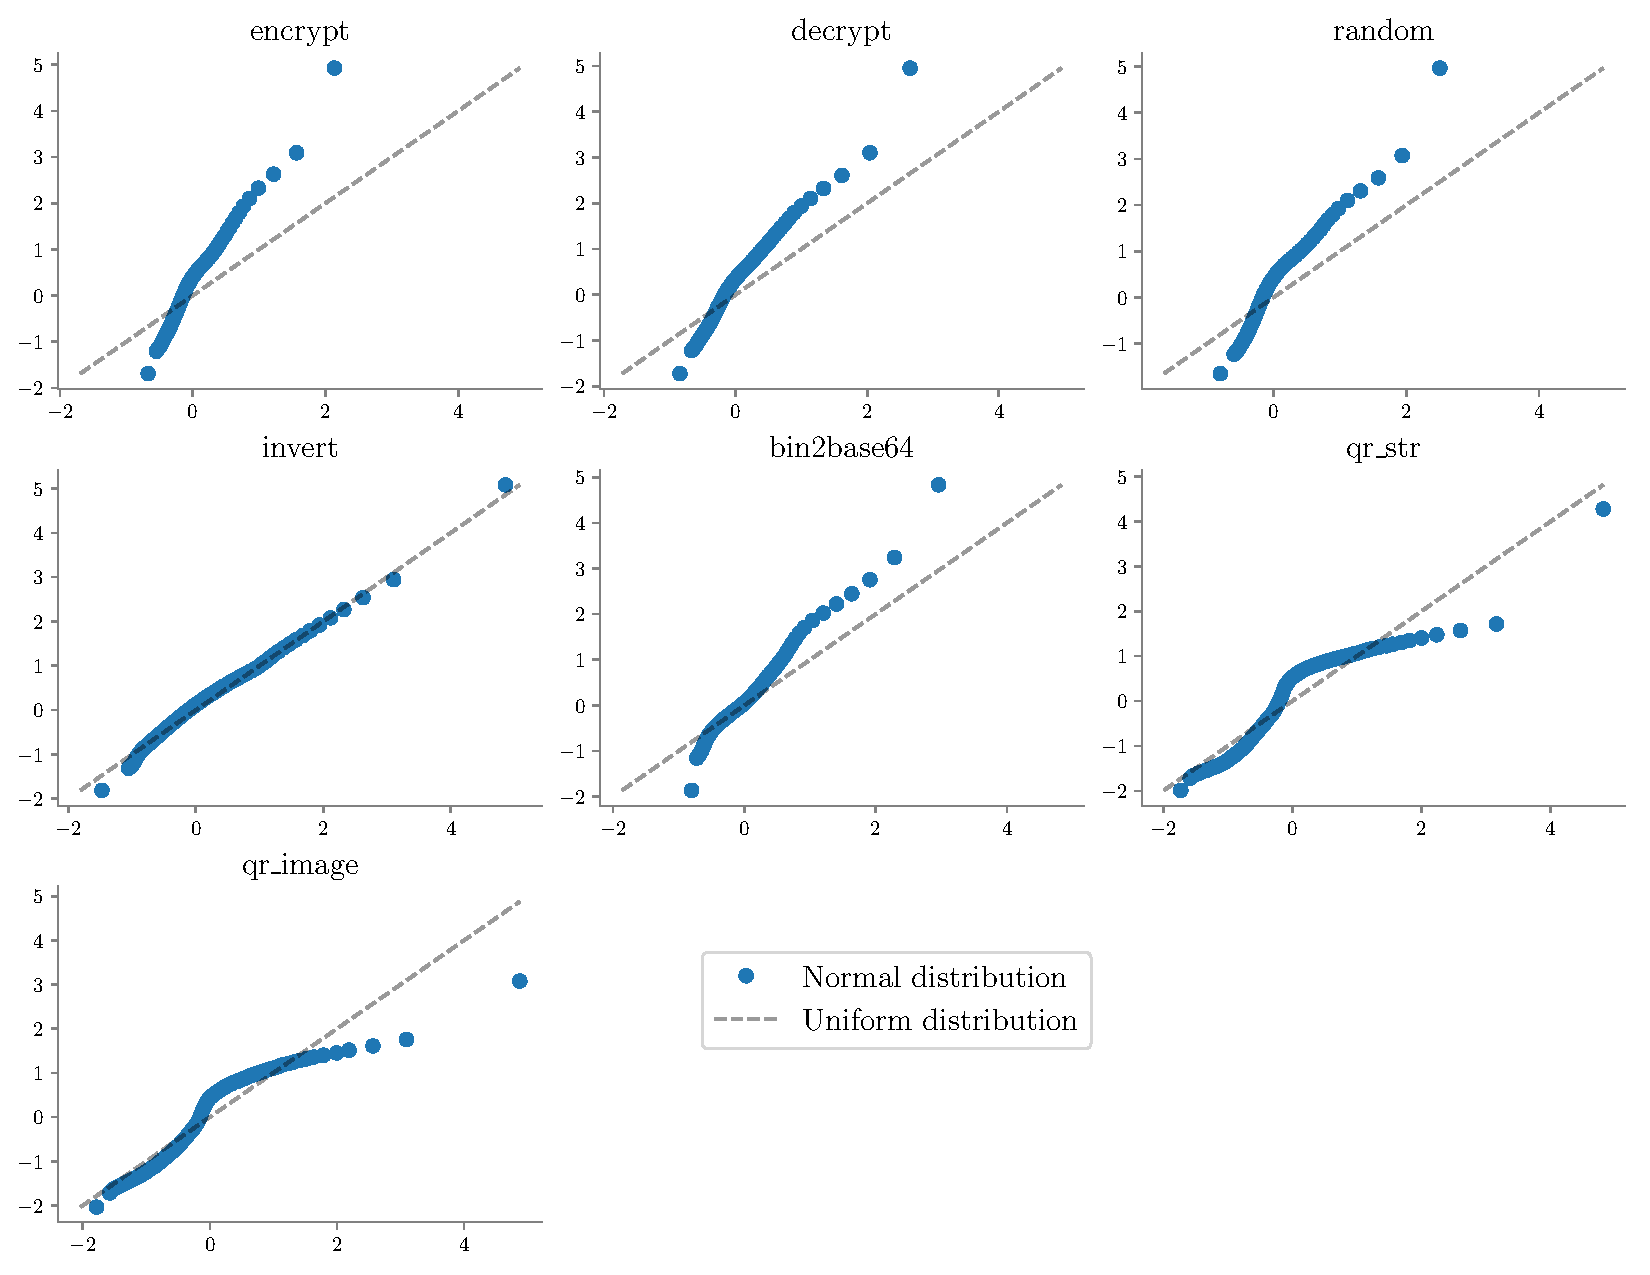
\includegraphics[width=\linewidth]{plots/qqplots.pdf}
    \caption{Execution time distributions. Each subplot represents the quantile-quantile plot of the two distributions, original and multivariant binary. }
    \label{rq3:diversity:times}
\end{figure*}



\begin{tcolorbox}[title=Answer to RQ3.,boxrule=2pt,arc=.3em,boxsep=1.5mm]
    
The execution time distributions are significantly different between the original and the multivariant binary. Furthermore, no specific variant can be inferred from execution times gathered from the multivariant binary. 
Consequently, attacks relying on measuring precise execution times \cite{blackhatpaper} of a function are made a lot harder to conduct as the distribution for the multivariant binary is different and even more spread than the original one.

\end{tcolorbox}
